\appendix
\section*{Apendix}

\addcontentsline{toc}{section}{APPENDIX}

\setcounter{table}{0} 
\renewcommand{\thetable}{A\arabic{table}}
\begin{center}
\begin{sidewaysfigure}[H]
\caption{Task Components}

\noindent\resizebox{\textwidth}{!}{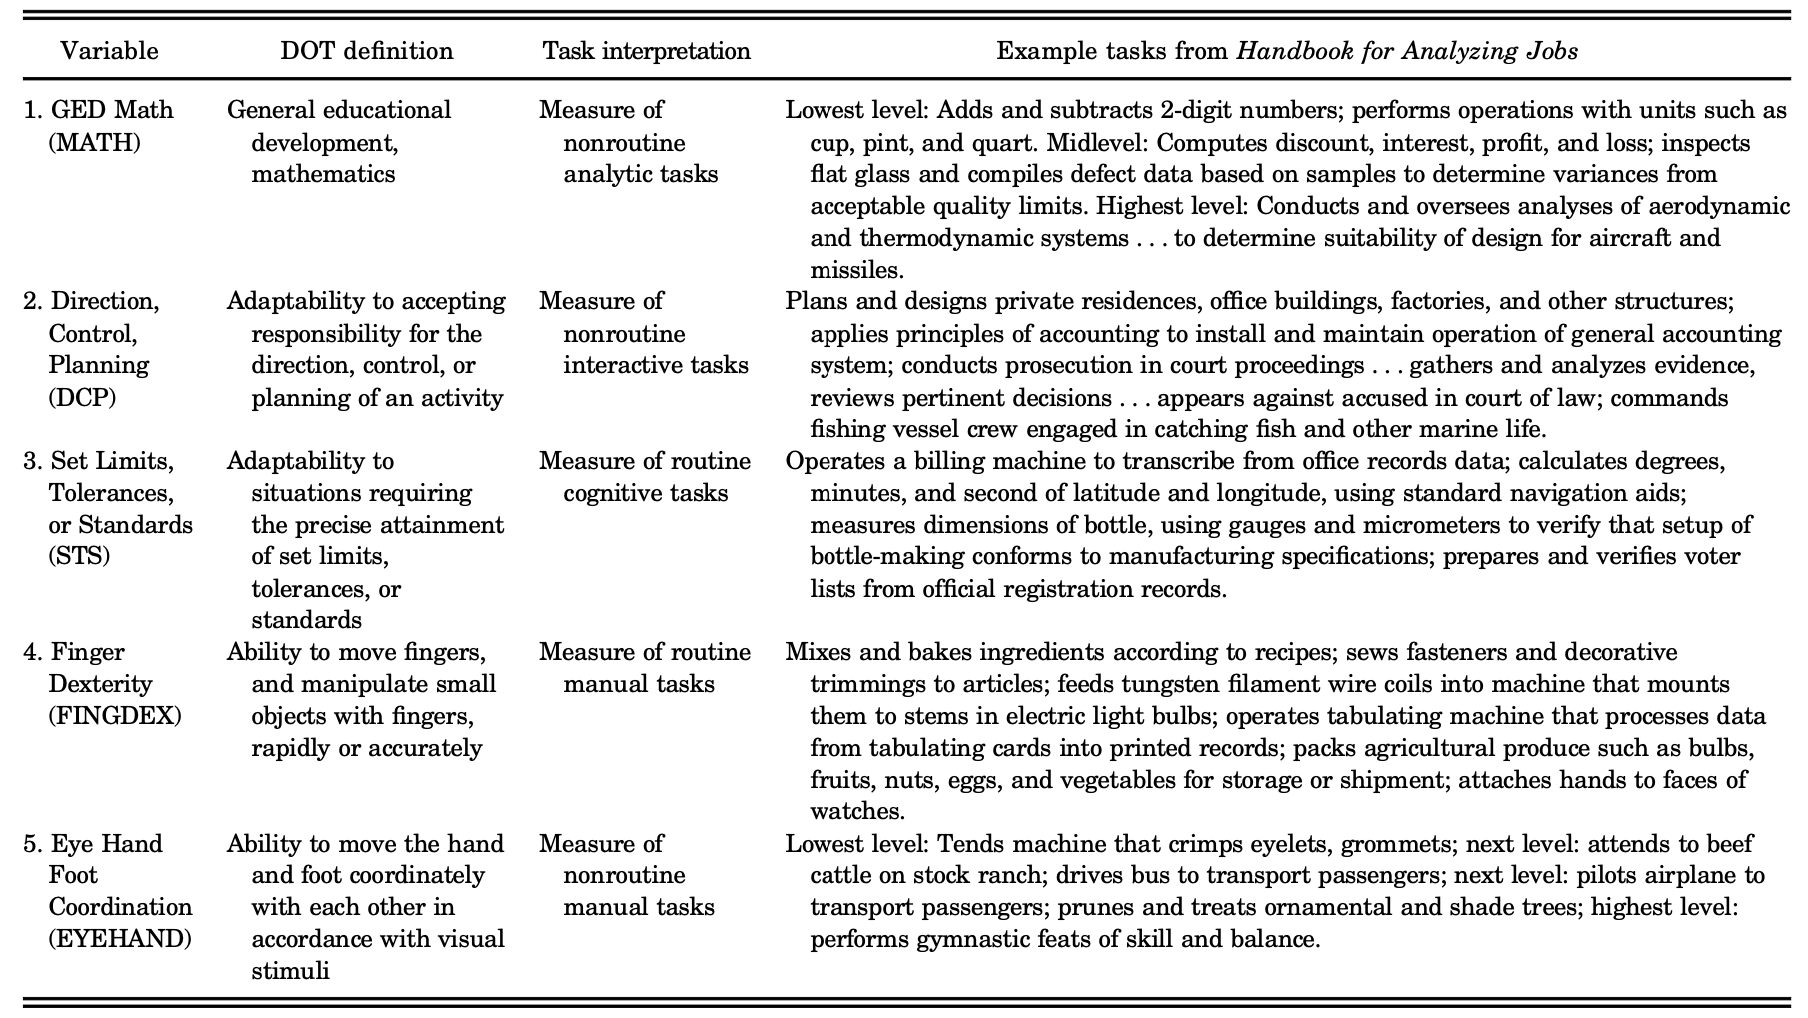
\includegraphics[width=0.95\textwidth]{figs/appendix/alm-2003-task-definitions.png}}

\textbf{Source: }Appendix of \citet{2003Autor}.

\begin{comment}
\medskip

\textbf{Source:} \citet{2003Autor}
\end{comment}
\end{sidewaysfigure}
\pagebreak
\par\end{center}

\begin{center}
\begin{figure}[H]
\begin{singlespace}
\begin{centering}
\caption{College/High-School Dynamics and Experience Interactions}
\par\end{centering}
\end{singlespace}
\begin{centering}
\subfloat[\label{fig:College/High-School-0-5-years}College/High-School Log
Relative Supply, 2004-2020 (0-5 Years of Experience)]{\begin{centering}
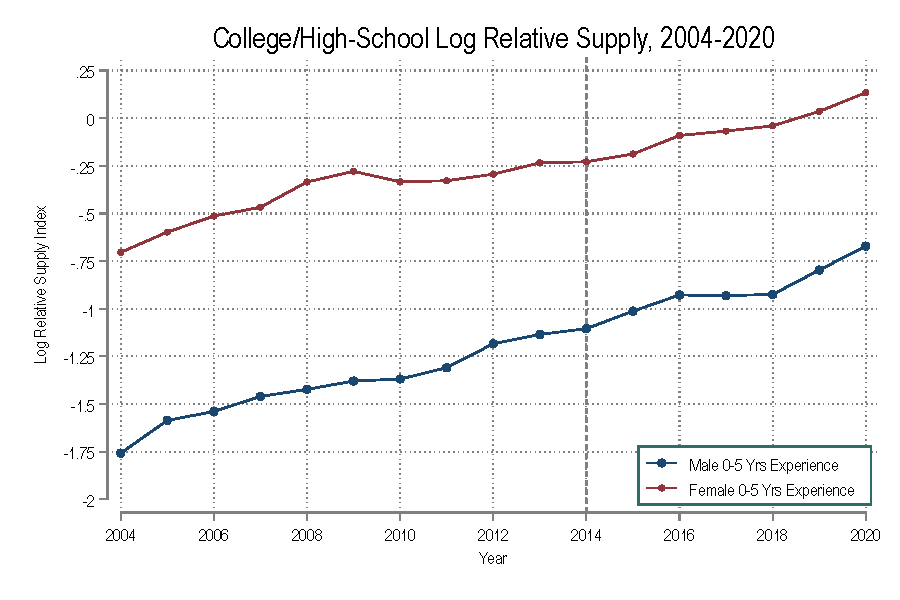
\includegraphics[width=0.75\textwidth,height=0.5\textwidth]{figs/appendix/college-hs-supply-exp-0-5.pdf}
\par\end{centering}
}
\par\end{centering}
\begin{centering}
\subfloat[\label{fig:College/High-School-11-15-years}College/High-School Log
Relative Supply, 2004-2020 (11-15 Years of Experience)]{\centering{}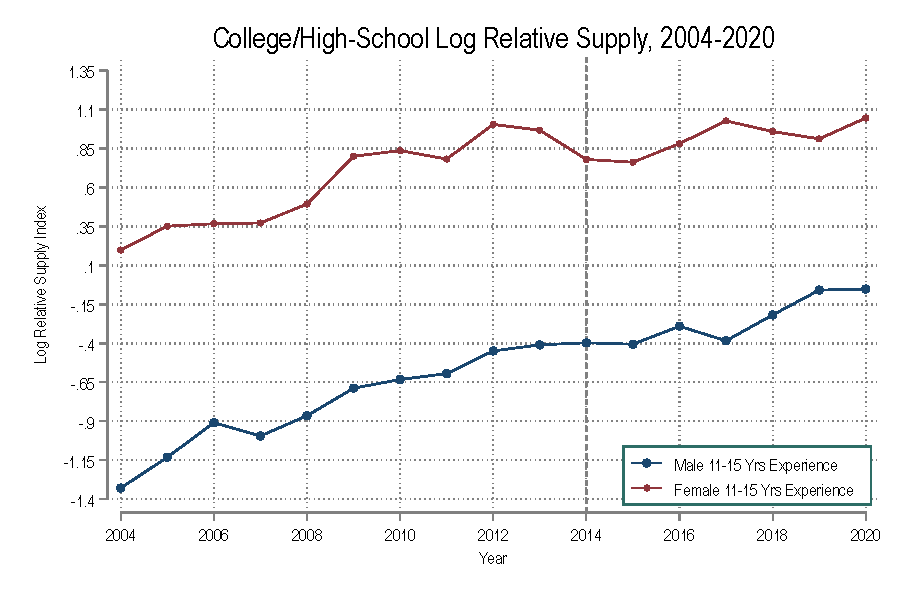
\includegraphics[width=0.75\textwidth,height=0.5\textwidth]{figs/appendix/college-hs-supply-exp-11-15.pdf}}
\par\end{centering}
\textbf{Source: }Author's calculations based on HLFS using efficiency
units. The log relative supply of females and males from different
experience levels.
\end{figure}
\par\end{center}

\begin{center}
\begin{figure}[H]
\begin{singlespace}
\caption{Employment Changes Across Major Industry Categories}

\end{singlespace}
\begin{singlespace}
\begin{centering}
\subfloat[Bar Plots]{\begin{centering}
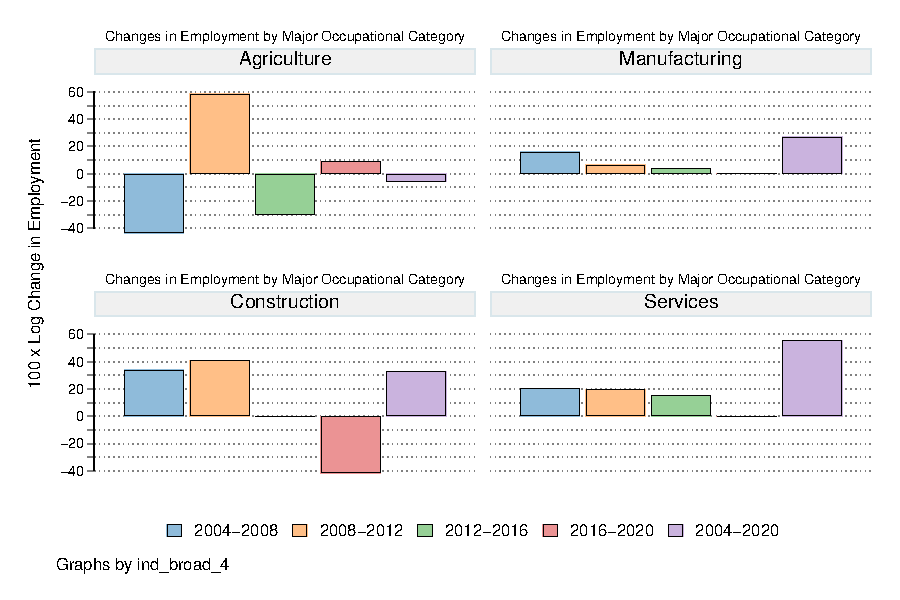
\includegraphics[scale=0.75]{figs/appendix/industry-employment-growth.pdf}
\par\end{centering}
}
\par\end{centering}
\end{singlespace}
\begin{centering}
\subfloat[Time Series Plot]{\begin{centering}
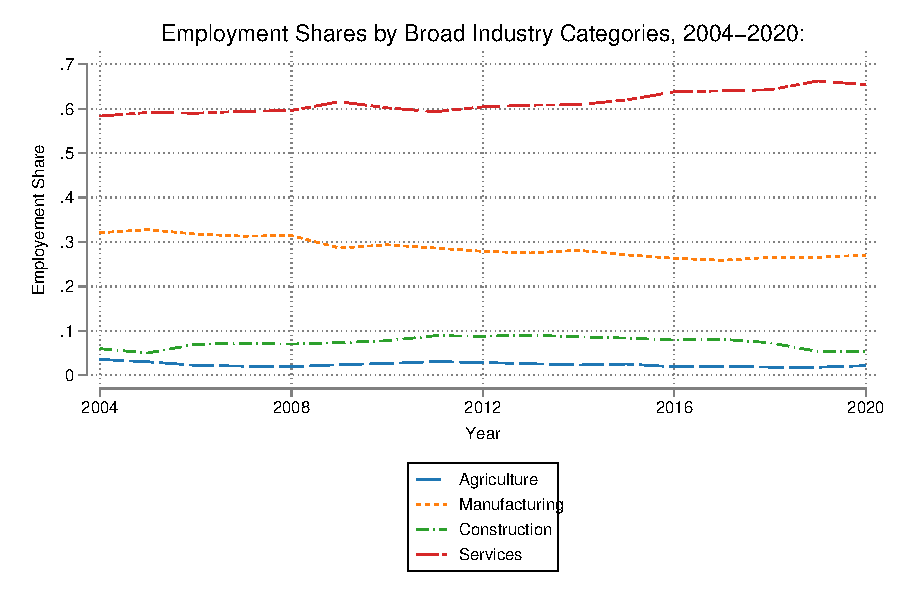
\includegraphics[scale=0.75]{figs/appendix/industry-employment-share-growth.pdf}
\par\end{centering}
\centering{}}
\par\end{centering}
\medskip

\textbf{Source: }Author's calculations based on the corresponding
waves of HLFS.
\end{figure}
 
\par\end{center}

\begin{center}
\begin{figure}[H]
\begin{singlespace}
\caption{Employment Shares of Major Occupational Groups}

\end{singlespace}
\begin{singlespace}
\begin{centering}
\subfloat[Employment Shares by 1-digit ISCO Occupation Classifications]{\begin{centering}
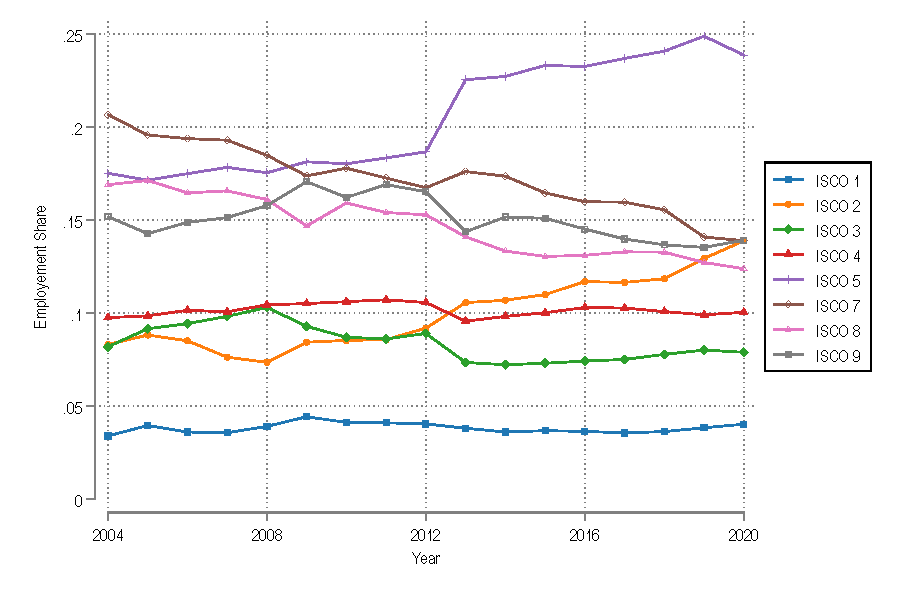
\includegraphics{figs/appendix/isco-1digit-employment-shares.pdf}
\par\end{centering}
}
\par\end{centering}
\end{singlespace}
\begin{centering}
\subfloat[Employment Shares by Broad Major Occupatinoal Groups]{\begin{centering}
\par\end{centering}
\centering{}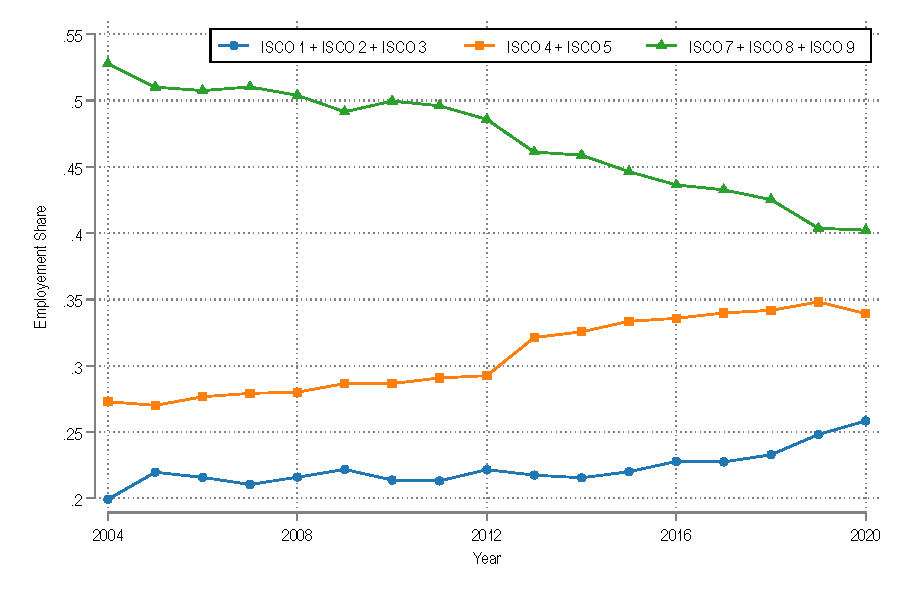
\includegraphics{figs/appendix/isco-broad-employment-shares.pdf}}
\par\end{centering}
\medskip

\textbf{Notes: }Author's calculations based on the corresponding waves
of HLFS.
\end{figure}
 
\par\end{center}

\begin{onehalfspace}
\begin{center}
\begin{figure}[H]
\begin{singlespace}
\caption{\label{fig:Composition-Adjusted-Educ-Cohorts-2}Composition Adjusted
Log Real Wages of Education Cohorts}

\end{singlespace}
\begin{singlespace}
\begin{centering}
\subfloat[Females Sample]{\begin{centering}
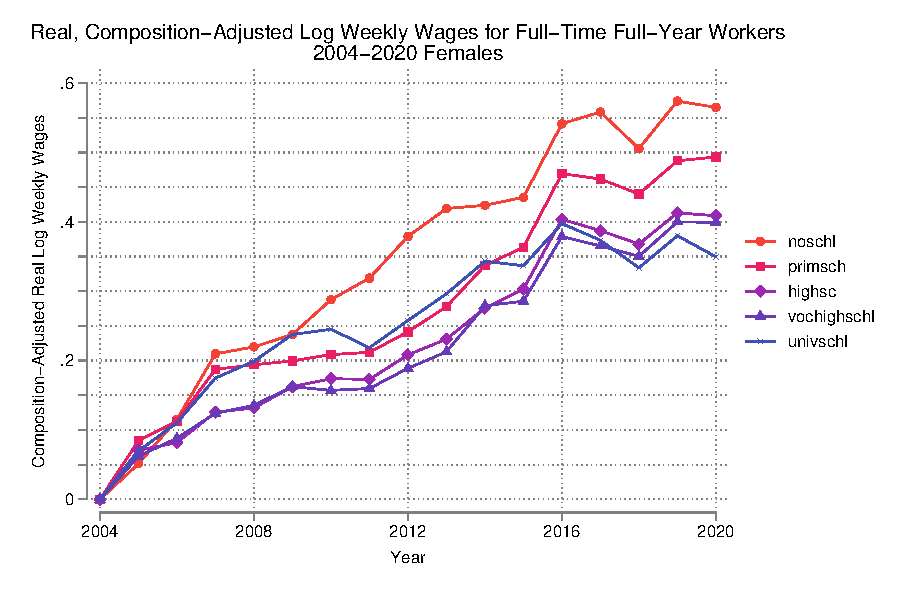
\includegraphics[width=1\textwidth,height=0.5\textwidth]{figs/appendix/comp-adj-log-wages-f-2004-2020.pdf}
\par\end{centering}
}
\par\end{centering}
\end{singlespace}
\begin{centering}
\subfloat[Males Sample]{\begin{centering}
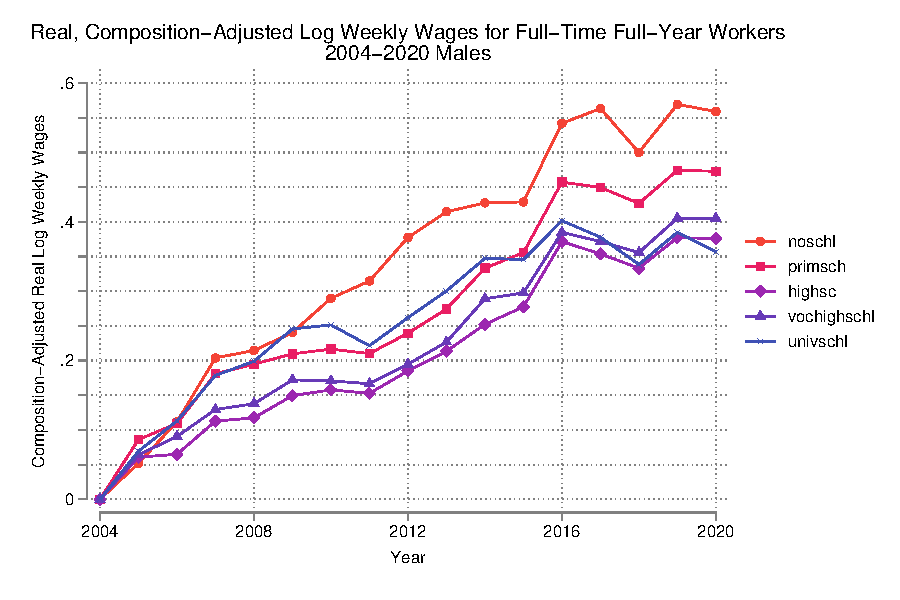
\includegraphics[width=1\textwidth,height=0.5\textwidth]{figs/appendix/comp-adj-log-wages-m-2004-2020.pdf}
\par\end{centering}
}
\par\end{centering}
\begin{singlespace}
\textbf{Source:} Authors's calculatiıons using HLFS (2004-2020).
Calculation of the labor supply is based on the reported usual weekly
working hours of all persons aged 14-64 who are employed and either
revieving a monthly wage or a salary. The real log weekly wages for
each education category is the weighted average of the relevant composition
adjusted cells using a fixed set of weights equal to the average employment
share of each group. Predicted nominal wages are deflated by the GDP
deflator. (noschl: below primary school, primsch: primary school,
highsc: high school, vochighschl: vocational high school, univschl:
college)
\end{singlespace}
\end{figure}
\par\end{center}
\end{onehalfspace}

\begin{center}
\begin{sidewaysfigure}[H]
\caption{Cross-sectional Relationship Between Mean Wages and Task Importance
Measures}

\centering{}\noindent\resizebox{\textheight}{!}{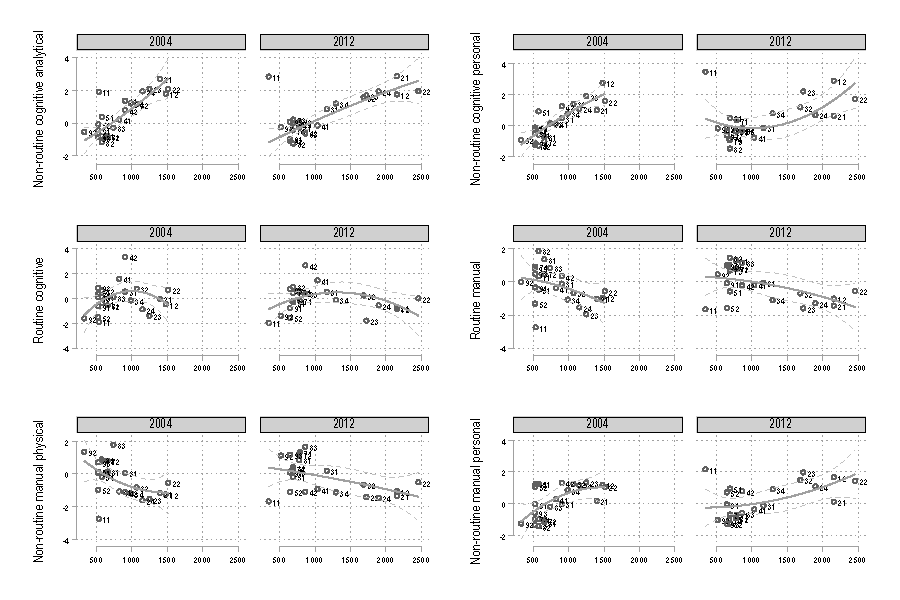
\includegraphics{figs/appendix/task-wage-relationship-2004-2012.pdf}}
\end{sidewaysfigure}
\par\end{center}

\begin{center}
\begin{figure}[H]
\caption{\label{fig:Country-Specific-Tasks}Country Specific Tasks}

\begin{centering}
\noindent\resizebox{\textwidth}{!}{%
\begin{tabular}{>{\raggedright}p{3cm}>{\centering}p{2cm}>{\centering}p{2cm}>{\centering}p{2cm}>{\centering}p{2cm}>{\centering}p{2cm}}
\toprule 
\textbf{Skill Categories} & \textbf{2- digit occupations} & \textbf{Non-routine cognitive analytical} & \textbf{Non-routine cognitive personal} & \textbf{Routine Cognitive} & \textbf{Routine Task Index}\tabularnewline
\midrule
Skilled & 11 & 0.11 & 0.01 & -0.47 & -0.43\tabularnewline
Skilled & 12 & 0.55 & 0.01 & 0.00 & -0.31\tabularnewline
Skilled & 13 & -0.29 & 0.21 & 0.23 & 0.28\tabularnewline
Skilled & 14 & 0.04 & -0.49 & 0.07 & 0.28\tabularnewline
Skilled & 21 & 0.62 & 0.34 & 0.36 & -0.16\tabularnewline
Skilled & 22 & 0.00 & 0.12 & 0.43 & 0.30\tabularnewline
Skilled & 23 & 0.62 & 1.31 & 0.34 & -0.52\tabularnewline
Skilled & 25 & 1.17 & 0.88 & -0.23 & -1.03\tabularnewline
Skilled & 26 & 0.44 & 1.29 & -0.01 & -0.67\tabularnewline
Skilled & 31 & -0.22 & -0.32 & 0.10 & 0.31\tabularnewline
Skilled & 32 & 0.03 & -0.12 & 0.15 & 0.18\tabularnewline
Skilled & 33 & -0.19 & -0.24 & 0.08 & 0.29\tabularnewline
Skilled & 34 & -0.05 & 0.44 & -0.47 & -0.43\tabularnewline
Skilled & 35 & 1.33 & -0.05 & -0.05 & -0.79\tabularnewline
\midrule Semi-skilled w.c & 41 & -0.02 & 0.25 & 0.21 & 0.10\tabularnewline
Semi-skilled w.c & 42 & 0.17 & -0.28 & 0.11 & 0.05\tabularnewline
Semi-skilled w.c & 43 & -0.07 & -0.26 & 0.13 & 0.30\tabularnewline
Semi-skilled w.c & 44 & 0.42 & -0.34 & -0.95 & -0.94\tabularnewline
Semi-skilled w.c & 51 & -0.24 & -0.35 & -0.31 & 0.02\tabularnewline
Semi-skilled w.c & 52 & -0.18 & -0.13 & -0.36 & -0.13\tabularnewline
Semi-skilled w.c & 53 & -0.58 & -0.14 & -0.68 & -0.15\tabularnewline
Semi-skilled w.c & 54 & -0.12 & 0.19 & 0.25 & 0.20\tabularnewline
\midrule Semi-skilled b.c & 61 & -0.37 & -0.36 & -0.27 & 0.12\tabularnewline
Semi-skilled b.c & 62 & -0.82 & -0.64 & -0.43 & 0.44\tabularnewline
Semi-skilled b.c & 63 & 0.42 & 1.60 & -0.95 & -1.51\tabularnewline
Semi-skilled b.c & 71 & -0.18 & -0.34 & -0.22 & 0.06\tabularnewline
Semi-skilled b.c & 72 & -0.09 & -0.45 & 0.02 & 0.21\tabularnewline
Semi-skilled b.c & 73 & -0.45 & 0.02 & -0.02 & 0.22\tabularnewline
Semi-skilled b.c & 74 & 0.17 & -0.10 & -0.31 & -0.33\tabularnewline
Semi-skilled b.c & 75 & 0.07 & -0.21 & 0.01 & 0.01\tabularnewline
Semi-skilled b.c & 81 & -0.36 & -0.32 & 0.30 & 0.51\tabularnewline
Semi-skilled b.c & 82 & -0.09 & -0.63 & 0.86 & 0.83\tabularnewline
Semi-skilled b.c & 83 & -0.02 & -0.18 & 0.23 & 0.22\tabularnewline
\midrule Elementary & 91 & 0.33 & -0.52 & -0.24 & -0.21\tabularnewline
Elementary & 92 & -0.29 & -0.15 & -0.52 & -0.19\tabularnewline
Elementary & 93 & -0.26 & -0.13 & 0.31 & 0.42\tabularnewline
Elementary & 94 & -0.05 & -0.70 & -0.31 & 0.02\tabularnewline
Elementary & 95 & 0.48 & -0.34 & -0.95 & -0.91\tabularnewline
Elementary & 96 & -0.48 & -0.28 & 0.14 & 0.49\tabularnewline
\bottomrule
\end{tabular}}
\par\end{centering}
\medskip

\textbf{Notes: }Author's calculations based on PIAAC data.
\end{figure}
\par\end{center}

\begin{center}
\begin{table}[H]
\caption{ISCO08 Occupational Codings}

\begin{centering}
\noindent\resizebox{\textwidth}{!}{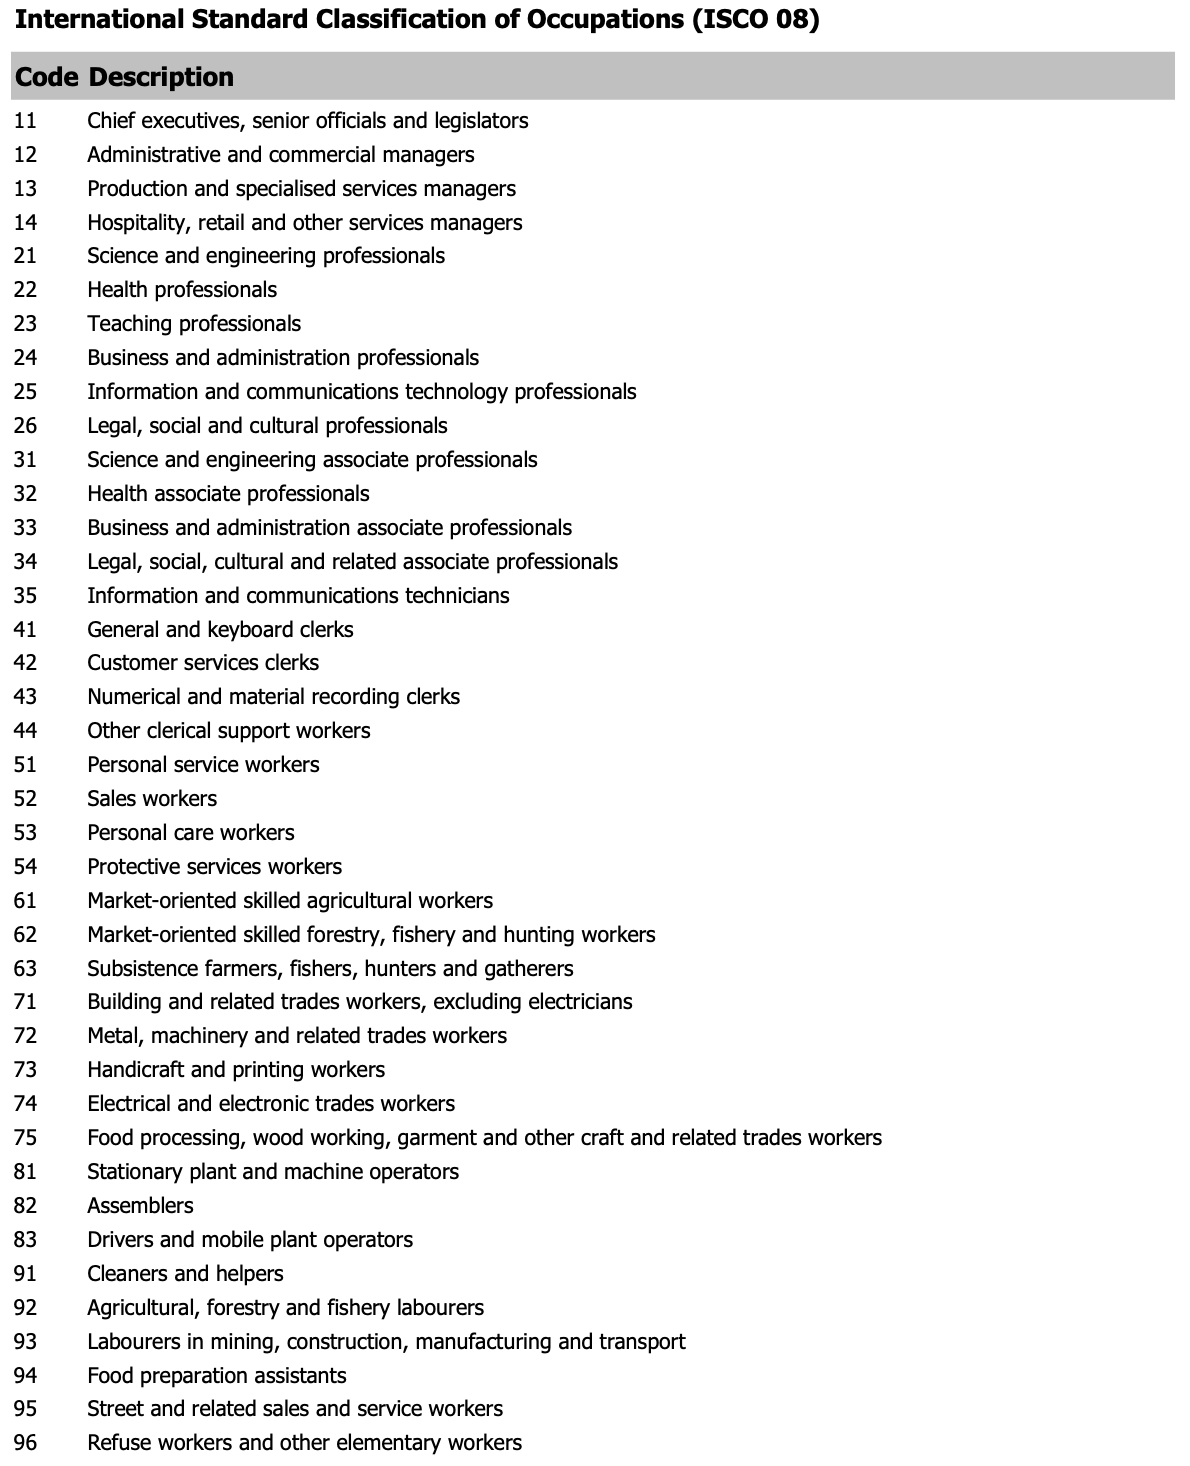
\includegraphics{figs/appendix/isco08-codes.png}}
\par\end{centering}
\medskip

\begin{singlespace}
\textbf{Source: }TurkStat
\end{singlespace}
\end{table}

\par\end{center}

\begin{center}
\begin{table}[H]
\caption{ISCO88 Occupational Codings}

\begin{centering}
\noindent\resizebox{\textwidth}{!}{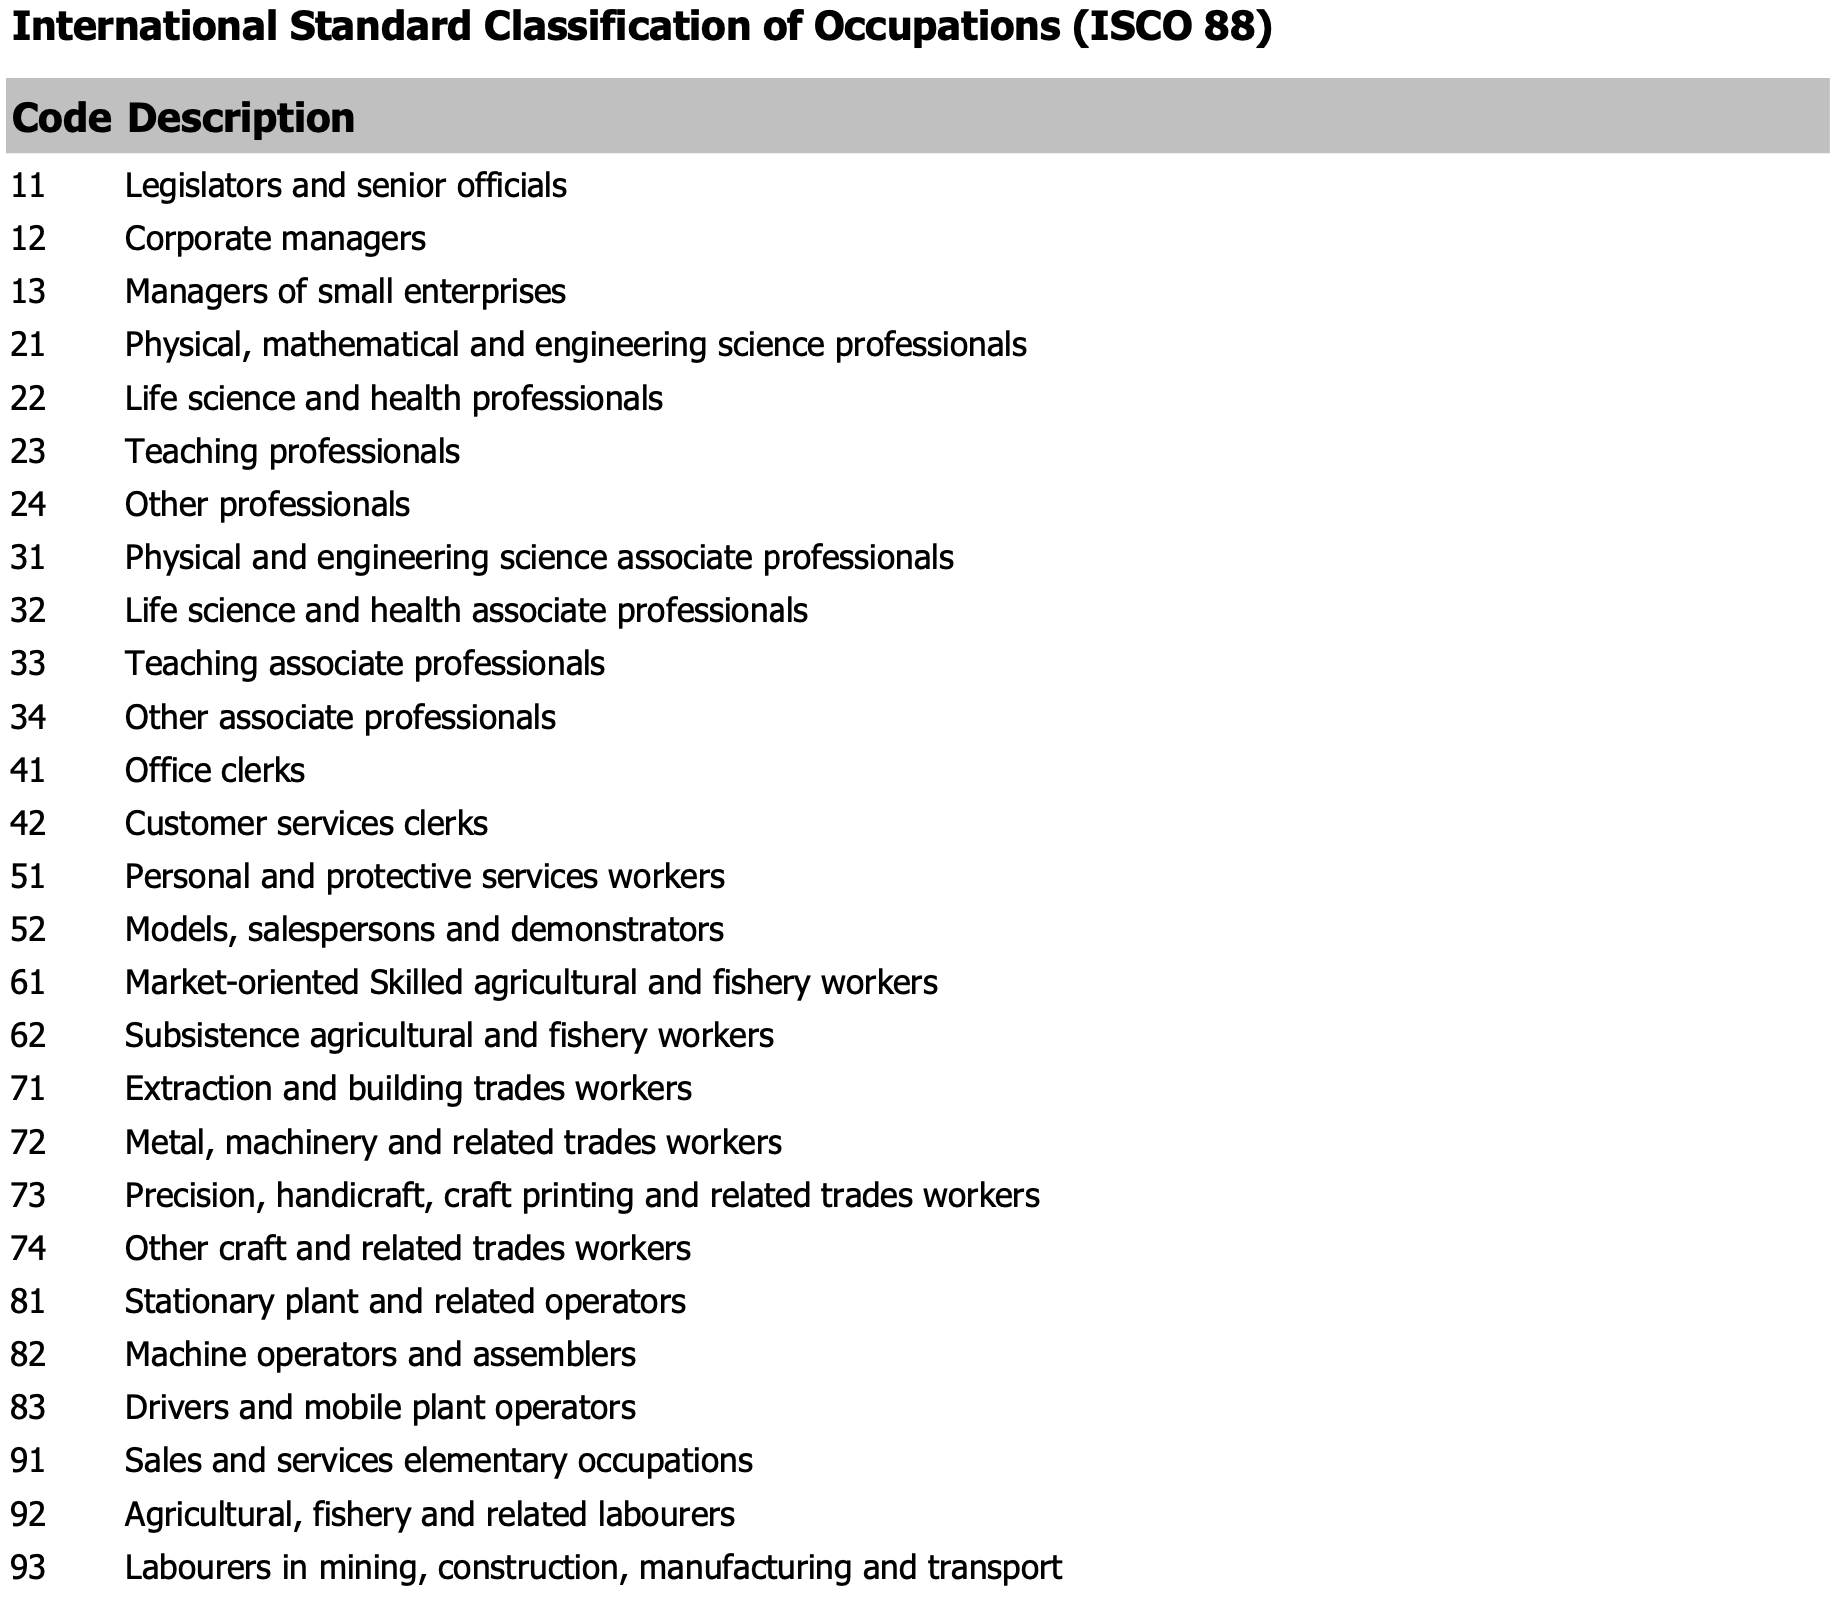
\includegraphics{figs/appendix/isco88-codes.png}}
\par\end{centering}
\medskip

\begin{singlespace}
\textbf{Source: }TurkStat
\end{singlespace}
\end{table}

\par\end{center}

\begin{singlespace}
\begin{center}
\begin{table}[H]
\begin{onehalfspace}
\caption{Means of O{*}NET task measures for four broad occupational groups
in 2015}

\end{onehalfspace}
\begin{centering}
\begin{tabular*}{1\textwidth}{@{\extracolsep{\fill}}l>{\centering}p{0.07\textwidth}>{\centering}p{0.07\textwidth}>{\centering}p{0.07\textwidth}>{\centering}p{0.07\textwidth}>{\centering}p{0.07\textwidth}>{\centering}p{0.07\textwidth}}
\toprule 
 & \textbf{All} & \textbf{Below Primary} & \textbf{Primary} & \textbf{High School} & \textbf{Voc. High School} & \textbf{College}\tabularnewline
\midrule 
\textbf{A. Females} & \multicolumn{6}{c}{}\tabularnewline
\midrule
\rowgroup{Non-routine cognitive} &  &  &  &  &  & \tabularnewline
\parbox{4cm}{Non-routine cognitive \\ analytical} & 0.12 & -0.45 & -0.60 & -0.26 & -0.03 & 1.08\tabularnewline
\parbox{4cm}{Non-routine cognitive \\ personal} & 0.11 & -0.23 & -0.42 & -0.15 & -0.03 & 0.82\tabularnewline
\rowgroup{Non-routine manual} &  &  &  &  &  & \tabularnewline
\parbox{4cm}{Non-routine manual \\ physical} & -0.48 & 0.12 & 0.09 & -0.54 & -0.51 & -1.12\tabularnewline
\parbox{4cm}{Non-routine manual \\ personal} & 0.27 & -0.04 & -0.31 & 0.13 & 0.28 & 0.94\tabularnewline
\rowgroup{Routine} &  &  &  &  &  & \tabularnewline
Routine cognitive & -0.15 & -0.72 & -0.28 & 0.34 & 0.35 & -0.25\tabularnewline
Routine manual & -0.36 & 0.08 & 0.23 & -0.33 & -0.33 & -1.03\tabularnewline
\rowgroup{Routine task intensity} & -0.18 & -0.16 & 0.24 & 0.30 & 0.17 & -0.85\tabularnewline
\midrule 
\textbf{B. Males} & \multicolumn{6}{c}{}\tabularnewline
\midrule
\rowgroup{Non-routine cognitive} &  &  &  &  &  & \tabularnewline
\parbox{4cm}{Non-routine cognitive \\ analytical} & -0.04 & -0.46 & -0.43 & -0.11 & -0.05 & 1.02\tabularnewline
\parbox{4cm}{Non-routine cognitive \\ personal} & -0.04 & -0.37 & -0.36 & 0.005 & -0.11 & 0.80\tabularnewline
\rowgroup{Non-routine manual} &  &  &  &  &  & \tabularnewline
\parbox{4cm}{Non-routine manual \\ physical} & 0.17 & 0.63 & 0.56 & 0.02 & 0.19 & -0.78\tabularnewline
\parbox{4cm}{Non-routine manual \\ personal} & -0.09 & -0.59 & -0.45 & 0.06 & -0.12 & 0.76\tabularnewline
\rowgroup{Routine} &  &  &  &  &  & \tabularnewline
Routine cognitive & 0.05 & -0.20 & 0.04 & 0.25 & 0.32 & -0.15\tabularnewline
Routine manual & 0.12 & 0.57 & 0.51 & -0.04 & 0.16 & -0.82\tabularnewline
\rowgroup{Routine task intensity} & 0.06 & 0.22 & 0.33 & 0.16 & 0.21 & -0.75\tabularnewline
\bottomrule
\end{tabular*}
\par\end{centering}
\medskip

\textbf{Source:} Author's calculations based on the framework introduced
by \citet{Acemoglu2011}.
\end{table}

\par\end{center}
\end{singlespace}

\begin{center}
\begin{table}[H]
\caption{\label{tab:Occupation's-Rank-by-RTI}Occupation's Rank by RTI Index
(2004)}

\begin{centering}
\begin{tabular}{cccccc}
\toprule 
Occupation & RTI & Weekly Wage & Level & Cumulative & Top 33\%\tabularnewline
\midrule 
82 & 1.60 & 2.48 & 9.05 & 9.05 & X\tabularnewline
74 & 1.41 & 2.32 & 7.52 & 16.57 & X\tabularnewline
81 & 1.21 & 2.53 & 1.37 & 17.94 & X\tabularnewline
73 & 1.16 & 2.50 & 1.13 & 19.07 & X\tabularnewline
41 & 0.78 & 2.85 & 7.62 & 26.69 & X\tabularnewline
72 & 0.55 & 2.65 & 5.95 & 32.64 & X\tabularnewline
42 & 0.46 & 2.92 & 2.63 & 35.27 & X\tabularnewline
93 & 0.25 & 2.36 & 4.05 & 39.32 & \tabularnewline
71 & 0.15 & 2.49 & 5.53 & 44.85 & \tabularnewline
91 & 0.03 & 2.41 & 7.36 & 52.21 & \tabularnewline
52 & -0.21 & 2.26 & 6.29 & 58.50 & \tabularnewline
61 & -0.25 & 2.36 & 0.51 & 59.01 & \tabularnewline
34 & -0.36 & 3.02 & 4.32 & 63.33 & \tabularnewline
24 & -0.61 & 3.21 & 2.50 & 65.83 & \tabularnewline
32 & -0.71 & 3.15 & 1.43 & 67.26 & \tabularnewline
51 & -0.79 & 2.55 & 10.43 & 77.69 & \tabularnewline
13 & -0.81 & 2.64 & 1.04 & 78.74 & \tabularnewline
21 & -0.86 & 3.40 & 1.25 & 79.99 & \tabularnewline
31 & -0.87 & 2.98 & 3.04 & 83.02 & \tabularnewline
83 & -0.91 & 2.57 & 8.25 & 91.27 & \tabularnewline
92 & -1.13 & 2.13 & 1.34 & 92.62 & \tabularnewline
12 & -1.18 & 3.44 & 2.55 & 95.17 & \tabularnewline
22 & -1.27 & 3.54 & 0.86 & 96.03 & \tabularnewline
23 & -2.27 & 3.53 & 3.97 & 100.00 & \tabularnewline
\bottomrule
\end{tabular}
\par\end{centering}
\medskip

\textbf{Source: }Author's calculations using HLFS.
\end{table}

\par\end{center}

\begin{center}
\begin{table}[H]
\caption{\label{tab:Task-Importance-Measures}Task Importance Measures}

\begin{centering}
\begin{tabular}{cr@{\extracolsep{0pt}.}lr@{\extracolsep{0pt}.}lr@{\extracolsep{0pt}.}lr@{\extracolsep{0pt}.}lr@{\extracolsep{0pt}.}lr@{\extracolsep{0pt}.}l}
\toprule 
ISCO & \multicolumn{2}{c}{NRCA} & \multicolumn{2}{c}{NRCP} & \multicolumn{2}{c}{RCOG} & \multicolumn{2}{c}{RMAN} & \multicolumn{2}{c}{NRMPHYS} & \multicolumn{2}{c}{NRMPERS}\tabularnewline
\midrule 
11 & 1&92 & -0&30 & -1&90 & -2&74 & -2&74 & 1&24\tabularnewline
12 & 1&80 & 2&77 & -0&47 & -0&96 & -1&26 & 1&17\tabularnewline
21 & 2&71 & 1&00 & -0&05 & -1&01 & -1&18 & 0&17\tabularnewline
22 & 2&09 & 1&58 & 0&70 & -0&57 & -0&54 & 1&05\tabularnewline
23 & 2&10 & 1&90 & -1&40 & -1&96 & -1&55 & 1&33\tabularnewline
24 & 1&94 & 1&08 & -0&88 & -1&54 & -1&62 & 1&14\tabularnewline
31 & 1&37 & 0&47 & 0&56 & -0&10 & 0&06 & -0&02\tabularnewline
32 & 1&16 & 1&40 & 0&79 & -0&67 & -0&83 & 1&25\tabularnewline
34 & 1&21 & 0&77 & -0&16 & -1&07 & -1&20 & 0&85\tabularnewline
41 & 0&21 & 0&10 & 1&58 & -0&37 & -1&07 & 0&27\tabularnewline
42 & 0&79 & 1&26 & 3&34 & 0&35 & -1&12 & 1&30\tabularnewline
51 & 0&37 & 0&92 & 0&14 & -0&46 & -0&18 & 1&24\tabularnewline
52 & -0&08 & -0&13 & -1&51 & -1&31 & -0&97 & 1&06\tabularnewline
71 & -0&78 & -0&58 & -0&37 & 0&34 & 0&81 & -0&99\tabularnewline
72 & -0&85 & -1&02 & -0&55 & 0&49 & 0&81 & -1&05\tabularnewline
73 & -0&69 & -1&27 & 0&11 & 0&50 & 0&11 & -1&34\tabularnewline
74 & -0&86 & -1&16 & 0&34 & 0&93 & 0&08 & -0&97\tabularnewline
81 & -0&80 & -0&75 & -0&55 & 1&38 & 0&14 & -1&19\tabularnewline
82 & -1&17 & -1&30 & 0&64 & 1&88 & 0&88 & -1&43\tabularnewline
83 & -0&29 & 0&14 & 0&10 & 0&85 & 1&78 & -0&19\tabularnewline
91 & -0&45 & -0&47 & -0&62 & -0&33 & 0&06 & -0&04\tabularnewline
92 & -0&55 & -0&93 & -1&61 & 0&00 & 1&35 & -1&26\tabularnewline
93 & -0&87 & -0&16 & 0&87 & 0&82 & 0&71 & -0&58\tabularnewline
\bottomrule
\end{tabular}
\par\end{centering}
\medskip

\textbf{Source: }Author's calculations using HLFS.
\end{table}

\par\end{center}

\begin{onehalfspace}
\begin{center}
\begin{sidewaystable}[H]
\caption{\label{tab:Polarization-Tests-rtipiaac-linear}Polarization Tests
for Jobs and Earnings}

\begin{centering}
\noindent\resizebox{\textwidth}{!}{%
\begin{tabular}{>{\raggedright}p{4cm}cccccccc}
\toprule 
 & \multicolumn{2}{c}{$\Delta$ in employment share} & \multicolumn{2}{c}{$\Delta$ in log mean real wage} & \multicolumn{2}{c}{$\Delta$ in employment share} & \multicolumn{2}{c}{$\Delta$ in log mean real wage}\tabularnewline
\cmidrule{2-9} \cmidrule{3-9} \cmidrule{4-9} \cmidrule{5-9} \cmidrule{6-9} \cmidrule{7-9} \cmidrule{8-9} \cmidrule{9-9} 
 & 2004/12 & 2012/22 & 2004/12 & 2012/22 & 2004/12 & 2012/22 & 2004/12 & 2012/22\tabularnewline
\cmidrule{2-9} \cmidrule{3-9} \cmidrule{4-9} \cmidrule{5-9} \cmidrule{6-9} \cmidrule{7-9} \cmidrule{8-9} \cmidrule{9-9} 
 & (1) & (2) & (3) & (4) & (5) & (6) & (7) & (8)\tabularnewline
RTI (O{*}NET) & -0.06{*} & -0.17 & -0.05{*} & 0.29{*}{*}{*} &  &  &  & \tabularnewline
 & (-2.73) & (-1.26) & (-2.20) & (4.50) &  &  &  & \tabularnewline
RTI (PIAAC) &  &  &  &  & -0.02 & -0.14 & -0.08 & 0.23{*}\tabularnewline
 &  &  &  &  & (-0.35) & (-0.88) & (-1.61) & (2.63)\tabularnewline
Constant & 0.00 & 0.08 & 0.41{*}{*}{*} & -0.05 & 0.01 & 0.04 & 0.41{*}{*}{*} & 0.02\tabularnewline
 & (0.14) & (0.77) & (12.09) & (-1.16) & (0.16) & (0.39) & (11.63) & (0.35)\tabularnewline
Observations & 22 & 32 & 22 & 32 & 22 & 32 & 22 & 32\tabularnewline
R-squared & 0.271 & 0.050 & 0.194 & 0.403 & 0.006 & 0.025 & 0.115 & 0.187\tabularnewline
Adjusted R-squared & 0.234 & 0.018 & 0.154 & 0.383 & -0.044 & -0.007 & 0.071 & 0.160\tabularnewline
\bottomrule
\end{tabular}}
\par\end{centering}
\medskip

\textbf{Notes:} t statistics in parentheses; {*} p<0.05,
{*}{*} p<0.01, {*}{*}{*} p<0.001
\end{sidewaystable}

\par\end{center}
\end{onehalfspace}

\begin{center}
\begin{table}[H]
\caption{\label{tab:Construction-of-task}Construction of task contents measures}

\begin{tabular}{>{\raggedright}m{0.25\textwidth}>{\raggedright}m{0.68\textwidth}}
\toprule 
Task Content Measure (\textbf{\textit{T}}) & Task Items (\textbf{\textit{J}})\tabularnewline
\midrule Non-routine cognitive analytical & Analyzing data/information (4.A.2.a.4)\tablefootnote{Codes in brackets corresponds to O{*}NET Work Activities, Work Context,
Abilities and Skills Importance scales. {[}\href{https://www.onetcenter.org/database.html\#all-files}{https://www.onetcenter.org/database.html\#all-files}{]}}

Thinking creatively (4.A.2.b.2)

Interpreting information for others (4.A.4.a.1)\tabularnewline
\midrule Non-routine cognitive interpersonal & Establishing and maintaining personal relationships (4.A.4.a.4)

Guiding, directing and motivating subordinates (4.A.4.b.4)

Coaching/developing others (4.A.4.b.5)\tabularnewline
\midrule Routine cognitive & The importance of repeating the same tasks (4.C.3.b.7)

The importance of being exact or accurate (4.C.3.b.4)

Structured vs. unstructured work (4.C.3.b.8)\tabularnewline
\midrule Routine manual & Pace determined by the speed of equipment (4.C.3.d.3)

Controlling machines and processes (4.A.3.a.3)

Spending time making repetitive motions (4.C.2.d.1.i)\tabularnewline
\midrule Non-routine manual physical & Operating vehicles, mechanized devices, or equipment (4.A.3.a.4)

Spending time using hands to handle, control or feel objects, tools
or controls (4.C.2.d.1.g)

Manual dexterity (1.A.2.a.2)

Spatial orientation (1.A.1.f.1)\tabularnewline
\bottomrule
\end{tabular} \medskip

\textbf{Notes:} Based on the elaborations of \citet{RePEc:eko:ekoeko:47_23},
who build the structure on the work of \citet{Acemoglu2011}.
\end{table}

\par\end{center}

\begin{center}
\begin{table}[h]
\caption{Occupation Coding Changes}

\begin{centering}
\begin{tabular}{c>{\centering}m{2cm}>{\centering}m{2cm}>{\centering}m{2cm}>{\centering}m{2cm}>{\centering}m{1.5cm}}
\toprule 
 & Regular Employee & Self-employed & Employer & \multicolumn{1}{>{\centering}m{2.5cm}}{Unpaid family worker} & Total\tabularnewline
\cmidrule{2-6} \cmidrule{3-6} \cmidrule{4-6} \cmidrule{5-6} \cmidrule{6-6} 
Observations & 651 & 2758 & 3381 & 13 & 6803\tabularnewline
Percentage & 15\% & 25\% & 35\% & 31\% & 100\%\tabularnewline
\bottomrule
\end{tabular}
\par\end{centering}
\medskip

\textbf{Source: }Author's calculations using HLFS.
\end{table}

\par\end{center}

\begin{center}
\begin{table}[H]
\caption{Correlation Table}

\begin{centering}
\noindent\resizebox{\textwidth}{!}{%
\begin{tabular}{lr@{\extracolsep{0pt}.}lr@{\extracolsep{0pt}.}lr@{\extracolsep{0pt}.}lr@{\extracolsep{0pt}.}lr@{\extracolsep{0pt}.}lr@{\extracolsep{0pt}.}lr@{\extracolsep{0pt}.}lr@{\extracolsep{0pt}.}lr@{\extracolsep{0pt}.}l}
\toprule 
 & \multicolumn{6}{l}{PIAAC (Individual-level)} & \multicolumn{6}{l}{PIAAC (Occupation-level)} & \multicolumn{6}{l}{O{*}NET (Occupation-level)}\tabularnewline
 & \multicolumn{2}{c}{Abstract} & \multicolumn{2}{c}{Routine} & \multicolumn{2}{c}{Manual} & \multicolumn{2}{c}{Abstract} & \multicolumn{2}{c}{Routine} & \multicolumn{2}{c}{Manual} & \multicolumn{2}{c}{Abstract} & \multicolumn{2}{c}{Routine} & \multicolumn{2}{c}{Manual}\tabularnewline
\cmidrule{2-19} \cmidrule{4-19} \cmidrule{6-19} \cmidrule{8-19} \cmidrule{10-19} \cmidrule{12-19} \cmidrule{14-19} \cmidrule{16-19} \cmidrule{18-19} 
\multicolumn{7}{l}{PIAAC (Individual-level)} & \multicolumn{2}{c}{} & \multicolumn{2}{c}{} & \multicolumn{2}{c}{} & \multicolumn{2}{c}{} & \multicolumn{2}{c}{} & \multicolumn{2}{c}{}\tabularnewline
Abstract & \multicolumn{2}{c}{1} & \multicolumn{2}{c}{} & \multicolumn{2}{c}{} & \multicolumn{2}{c}{} & \multicolumn{2}{c}{} & \multicolumn{2}{c}{} & \multicolumn{2}{c}{} & \multicolumn{2}{c}{} & \multicolumn{2}{c}{}\tabularnewline
Routine & -0&700 & \multicolumn{2}{c}{1} & \multicolumn{2}{c}{} & \multicolumn{2}{c}{} & \multicolumn{2}{c}{} & \multicolumn{2}{c}{} & \multicolumn{2}{c}{} & \multicolumn{2}{c}{} & \multicolumn{2}{c}{}\tabularnewline
Manual & -0&103 & 0&098 & \multicolumn{2}{c}{1} & \multicolumn{2}{c}{} & \multicolumn{2}{c}{} & \multicolumn{2}{c}{} & \multicolumn{2}{c}{} & \multicolumn{2}{c}{} & \multicolumn{2}{c}{}\tabularnewline
\multicolumn{7}{l}{PIAAC (Occupation-level)} & \multicolumn{2}{c}{} & \multicolumn{2}{c}{} & \multicolumn{2}{c}{} & \multicolumn{2}{c}{} & \multicolumn{2}{c}{} & \multicolumn{2}{c}{}\tabularnewline
Abstract & 0&535 & -0&492 & -0&325 & \multicolumn{2}{c}{1} & \multicolumn{2}{c}{} & \multicolumn{2}{c}{} & \multicolumn{2}{c}{} & \multicolumn{2}{c}{} & \multicolumn{2}{c}{}\tabularnewline
Routine & -0&495 & 0&532 & 0&294 & -0&926 & \multicolumn{2}{c}{1} & \multicolumn{2}{c}{} & \multicolumn{2}{c}{} & \multicolumn{2}{c}{} & \multicolumn{2}{c}{}\tabularnewline
Manual & -0&347 & 0&313 & 0&500 & -0&649 & 0&589 & \multicolumn{2}{c}{1} & \multicolumn{2}{c}{} & \multicolumn{2}{c}{} & \multicolumn{2}{c}{}\tabularnewline
\multicolumn{7}{l}{O{*}NET (Occupation-level)} & \multicolumn{2}{c}{} & \multicolumn{2}{c}{} & \multicolumn{2}{c}{} & \multicolumn{2}{c}{} & \multicolumn{2}{c}{} & \multicolumn{2}{c}{}\tabularnewline
Abstract & 0&394 & -0&399 & -0&330 & 0&736 & -0&750 & -0&660 & \multicolumn{2}{c}{1} & \multicolumn{2}{c}{} & \multicolumn{2}{c}{}\tabularnewline
Routine & -0&356 & 0&389 & 0&272 & -0&666 & 0&732 & 0&544 & -0&759 & \multicolumn{2}{c}{1} & \multicolumn{2}{c}{}\tabularnewline
Manual & -0&417 & 0&405 & 0&388 & -0&778 & 0&762 & 0&774 & -0&796 & 0&789 & \multicolumn{2}{c}{1}\tabularnewline
\bottomrule
\end{tabular}}
\par\end{centering}
\medskip

\textbf{Source: }Author's calculations using HLFS.
\end{table}

\par\end{center}

\begin{center}
\begin{table}[H]
\caption{\label{tab:Allocation-Between-Occupations-and-tasks}Allocation Between
Occupations And Tasks}

\begin{singlespace}
\begin{centering}
\noindent\resizebox{\textwidth}{!}{{\footnotesize{}}%
\begin{tabular*}{1\textwidth}{@{\extracolsep{\fill}}>{\raggedright}p{0.5cm}l>{\raggedleft}p{0.75cm}@{\extracolsep{0pt}.}p{0.75cm}l>{\raggedleft}p{0.025\columnwidth}@{\extracolsep{0pt}.}p{0.025\columnwidth}>{\raggedleft}p{0.5cm}@{\extracolsep{0pt}.}p{0.5cm}>{\raggedleft}p{0.5cm}@{\extracolsep{0pt}.}p{0.5cm}}
\toprule 
{\footnotesize{}ISCO} & Occupations & {\footnotesize{}Emp}&{\footnotesize{} Share 2004} & {\footnotesize{}Task} & \multicolumn{2}{p{0.05\columnwidth}}{{\footnotesize{}Change in}} & {\footnotesize{}Emp Sh}& & \multicolumn{2}{p{1cm}}{{\footnotesize{}2004-2012}}\tabularnewline
\midrule
 & \textbf{\footnotesize{}Technical and Professional} & \multicolumn{2}{p{1.5cm}}{} &  & \multicolumn{2}{p{0.05\columnwidth}}{{\footnotesize{}all}} & \multicolumn{2}{p{1cm}}{{\footnotesize{}manuf}} & \multicolumn{2}{p{1cm}}{{\footnotesize{}serv}}\tabularnewline
{\footnotesize{}21} & {\footnotesize{}Physical, mathematical and eng prof.} & {\footnotesize{}1}&{\footnotesize{}1} & {\footnotesize{}NR Cog.} & {\footnotesize{}0}&{\footnotesize{}5} & {\footnotesize{}0}&{\footnotesize{}5} & {\footnotesize{}0}&{\footnotesize{}5}\tabularnewline
{\footnotesize{}23} & {\footnotesize{}Teaching professionals} & {\footnotesize{}3}&{\footnotesize{}9} & {\footnotesize{}NR Cog.} & {\footnotesize{}-0}&{\footnotesize{}5} & {\footnotesize{}0}&{\footnotesize{}0} & {\footnotesize{}-1}&{\footnotesize{}3}\tabularnewline
{\footnotesize{}24} & {\footnotesize{}Other professionals} & {\footnotesize{}2}&{\footnotesize{}3} & {\footnotesize{}NR Cog.} & {\footnotesize{}0}&{\footnotesize{}4} & {\footnotesize{}-0}&{\footnotesize{}1} & {\footnotesize{}0}&{\footnotesize{}5}\tabularnewline
{\footnotesize{}31} & {\footnotesize{}Physical, mathematical and eng. assoc.} & {\footnotesize{}2}&{\footnotesize{}7} & {\footnotesize{}NR Cog.} & {\footnotesize{}0}&{\footnotesize{}2} & {\footnotesize{}0}&{\footnotesize{}9} & {\footnotesize{}0}&{\footnotesize{}0}\tabularnewline
{\footnotesize{}34} & {\footnotesize{}Teaching associate professionals} & {\footnotesize{}3}&{\footnotesize{}6} & {\footnotesize{}NR Cog.} & {\footnotesize{}0}&{\footnotesize{}7} & {\footnotesize{}0}&{\footnotesize{}2} & {\footnotesize{}0}&{\footnotesize{}9}\tabularnewline
 & \textbf{\footnotesize{}Managerial and Health Proff.} & \multicolumn{2}{p{1.5cm}}{} &  & \multicolumn{2}{p{0.05\columnwidth}}{} & \multicolumn{2}{p{1cm}}{} & \multicolumn{2}{p{1cm}}{}\tabularnewline
{\footnotesize{}11} & {\footnotesize{}Legislators and senior officials} & {\footnotesize{}0}&{\footnotesize{}6} & {\footnotesize{}NR Cog.} & {\footnotesize{}-0}&{\footnotesize{}4} & {\footnotesize{}0}&{\footnotesize{}0} & {\footnotesize{}-0}&{\footnotesize{}8}\tabularnewline
{\footnotesize{}12} & {\footnotesize{}Corporate managers} & {\footnotesize{}2}&{\footnotesize{}2} & {\footnotesize{}NR Pers.} & {\footnotesize{}0}&{\footnotesize{}9} & {\footnotesize{}1}&{\footnotesize{}0} & {\footnotesize{}0}&{\footnotesize{}8}\tabularnewline
{\footnotesize{}22} & {\footnotesize{}Life science and health prof.} & {\footnotesize{}0}&{\footnotesize{}9} & {\footnotesize{}NR Cog.} & {\footnotesize{}0}&{\footnotesize{}6} & {\footnotesize{}0}&{\footnotesize{}1} & {\footnotesize{}0}&{\footnotesize{}8}\tabularnewline
{\footnotesize{}32} & {\footnotesize{}Life science and health assoc. prof.} & {\footnotesize{}1}&{\footnotesize{}6} & {\footnotesize{}NR Pers.} & {\footnotesize{}-0}&{\footnotesize{}3} & {\footnotesize{}0}&{\footnotesize{}0} & {\footnotesize{}-0}&{\footnotesize{}6}\tabularnewline
\multicolumn{1}{l}{{\footnotesize{}41}} & \textbf{\footnotesize{}Office Clerks} & {\footnotesize{}7}&{\footnotesize{}0} & {\footnotesize{}R. Cog} & {\footnotesize{}-0}&{\footnotesize{}3} & {\footnotesize{}0}&{\footnotesize{}3} & {\footnotesize{}-0}&{\footnotesize{}9}\tabularnewline
{\footnotesize{}51} & \textbf{\footnotesize{}Personal and Protective Services} & {\footnotesize{}11}&{\footnotesize{}3} & {\footnotesize{}NRM Pers.} & {\footnotesize{}-0}&{\footnotesize{}2} & {\footnotesize{}-1}&{\footnotesize{}0} & {\footnotesize{}-0}&{\footnotesize{}8}\tabularnewline
 & \textbf{\footnotesize{}Sales ticket clerks and other services} & \multicolumn{2}{p{1.5cm}}{} &  & \multicolumn{2}{p{0.05\columnwidth}}{} & \multicolumn{2}{p{1cm}}{} & \multicolumn{2}{p{1cm}}{}\tabularnewline
{\footnotesize{}42} & {\footnotesize{}Customer services clerks} & {\footnotesize{}2}&{\footnotesize{}4} & {\footnotesize{}R. Cog.} & {\footnotesize{}0}&{\footnotesize{}4} & {\footnotesize{}0}&{\footnotesize{}0} & {\footnotesize{}0}&{\footnotesize{}4}\tabularnewline
{\footnotesize{}52} & {\footnotesize{}Models and salespersons} & {\footnotesize{}6}&{\footnotesize{}3} & {\footnotesize{}NRM Pers} & {\footnotesize{}1}&{\footnotesize{}4} & {\footnotesize{}0}&{\footnotesize{}3} & {\footnotesize{}1}&{\footnotesize{}6}\tabularnewline
{\footnotesize{}91} & {\footnotesize{}Sales and services elementary occs.} & {\footnotesize{}7}&{\footnotesize{}9} & {\footnotesize{}NRM Phys.} & {\footnotesize{}0}&{\footnotesize{}4} & {\footnotesize{}0}&{\footnotesize{}1} & {\footnotesize{}0}&{\footnotesize{}2}\tabularnewline
 & \textbf{\footnotesize{}Routine Operators} & \multicolumn{2}{p{1.5cm}}{} &  & \multicolumn{2}{p{0.05\columnwidth}}{} & \multicolumn{2}{p{1cm}}{} & \multicolumn{2}{p{1cm}}{}\tabularnewline
{\footnotesize{}73} & {\footnotesize{}Precision, handicraft and related} & {\footnotesize{}1}&{\footnotesize{}1} & {\footnotesize{}R. Man.} & {\footnotesize{}-0}&{\footnotesize{}2} & {\footnotesize{}-0}&{\footnotesize{}2} & {\footnotesize{}0}&{\footnotesize{}1}\tabularnewline
{\footnotesize{}74} & {\footnotesize{}Other craft and related trade work.} & {\footnotesize{}7}&{\footnotesize{}8} & {\footnotesize{}R. Man.} & {\footnotesize{}-2}&{\footnotesize{}4} & {\footnotesize{}-5}&{\footnotesize{}1} & {\footnotesize{}-0}&{\footnotesize{}1}\tabularnewline
{\footnotesize{}81} & {\footnotesize{}Stationary-plant and related operators} & {\footnotesize{}1}&{\footnotesize{}3} & {\footnotesize{}R. Man.} & {\footnotesize{}-0}&{\footnotesize{}3} & {\footnotesize{}-0}&{\footnotesize{}2} & {\footnotesize{}-0}&{\footnotesize{}1}\tabularnewline
{\footnotesize{}82} & {\footnotesize{}Machine operators and assemblers} & {\footnotesize{}7}&{\footnotesize{}6} & {\footnotesize{}R. Man.} & {\footnotesize{}-1}&{\footnotesize{}0} & {\footnotesize{}0}&{\footnotesize{}1} & {\footnotesize{}-0}&{\footnotesize{}1}\tabularnewline
 & \textbf{\footnotesize{}Operators} & \multicolumn{2}{p{1.5cm}}{} &  & \multicolumn{2}{p{0.05\columnwidth}}{} & \multicolumn{2}{p{1cm}}{} & \multicolumn{2}{p{1cm}}{}\tabularnewline
{\footnotesize{}71} & {\footnotesize{}Extraction and building trades} & {\footnotesize{}6}&{\footnotesize{}4} & {\footnotesize{}NRM Phys.} & {\footnotesize{}-0}&{\footnotesize{}7} & {\footnotesize{}-0}&{\footnotesize{}6} & {\footnotesize{}-0}&{\footnotesize{}2}\tabularnewline
{\footnotesize{}72} & {\footnotesize{}Metal, machinery and related} & {\footnotesize{}6}&{\footnotesize{}3} & {\footnotesize{}NRM Phys.} & {\footnotesize{}-0}&{\footnotesize{}5} & {\footnotesize{}0}&{\footnotesize{}1} & {\footnotesize{}-0}&{\footnotesize{}5}\tabularnewline
{\footnotesize{}83} & {\footnotesize{}Drivers and mobile-plant operators} & {\footnotesize{}7}&{\footnotesize{}7} & {\footnotesize{}NRM Phys.} & {\footnotesize{}0}&{\footnotesize{}3} & {\footnotesize{}0}&{\footnotesize{}3} & {\footnotesize{}-0}&{\footnotesize{}1}\tabularnewline
{\footnotesize{}92} & {\footnotesize{}Agricultural, fishery laborers} & {\footnotesize{}3}&{\footnotesize{}2} & {\footnotesize{}NRM Phys.} & {\footnotesize{}0}&{\footnotesize{}8} & {\footnotesize{}0}&{\footnotesize{}0} & {\footnotesize{}-0}&{\footnotesize{}1}\tabularnewline
\bottomrule
\end{tabular*}{\footnotesize{}}}{\footnotesize\par}
\par\end{centering}
\end{singlespace}
\medskip

\textbf{Source: }Author's calculations based on the O{*}NET data and
two waves of HLFS data (2004, 2012).
\end{table}

\par\end{center}

\newpage{}
\begin{center}
\begin{sidewaystable}[H]
\begin{centering}
\caption{ISCO88 and ISCO08 Transition Matrix}
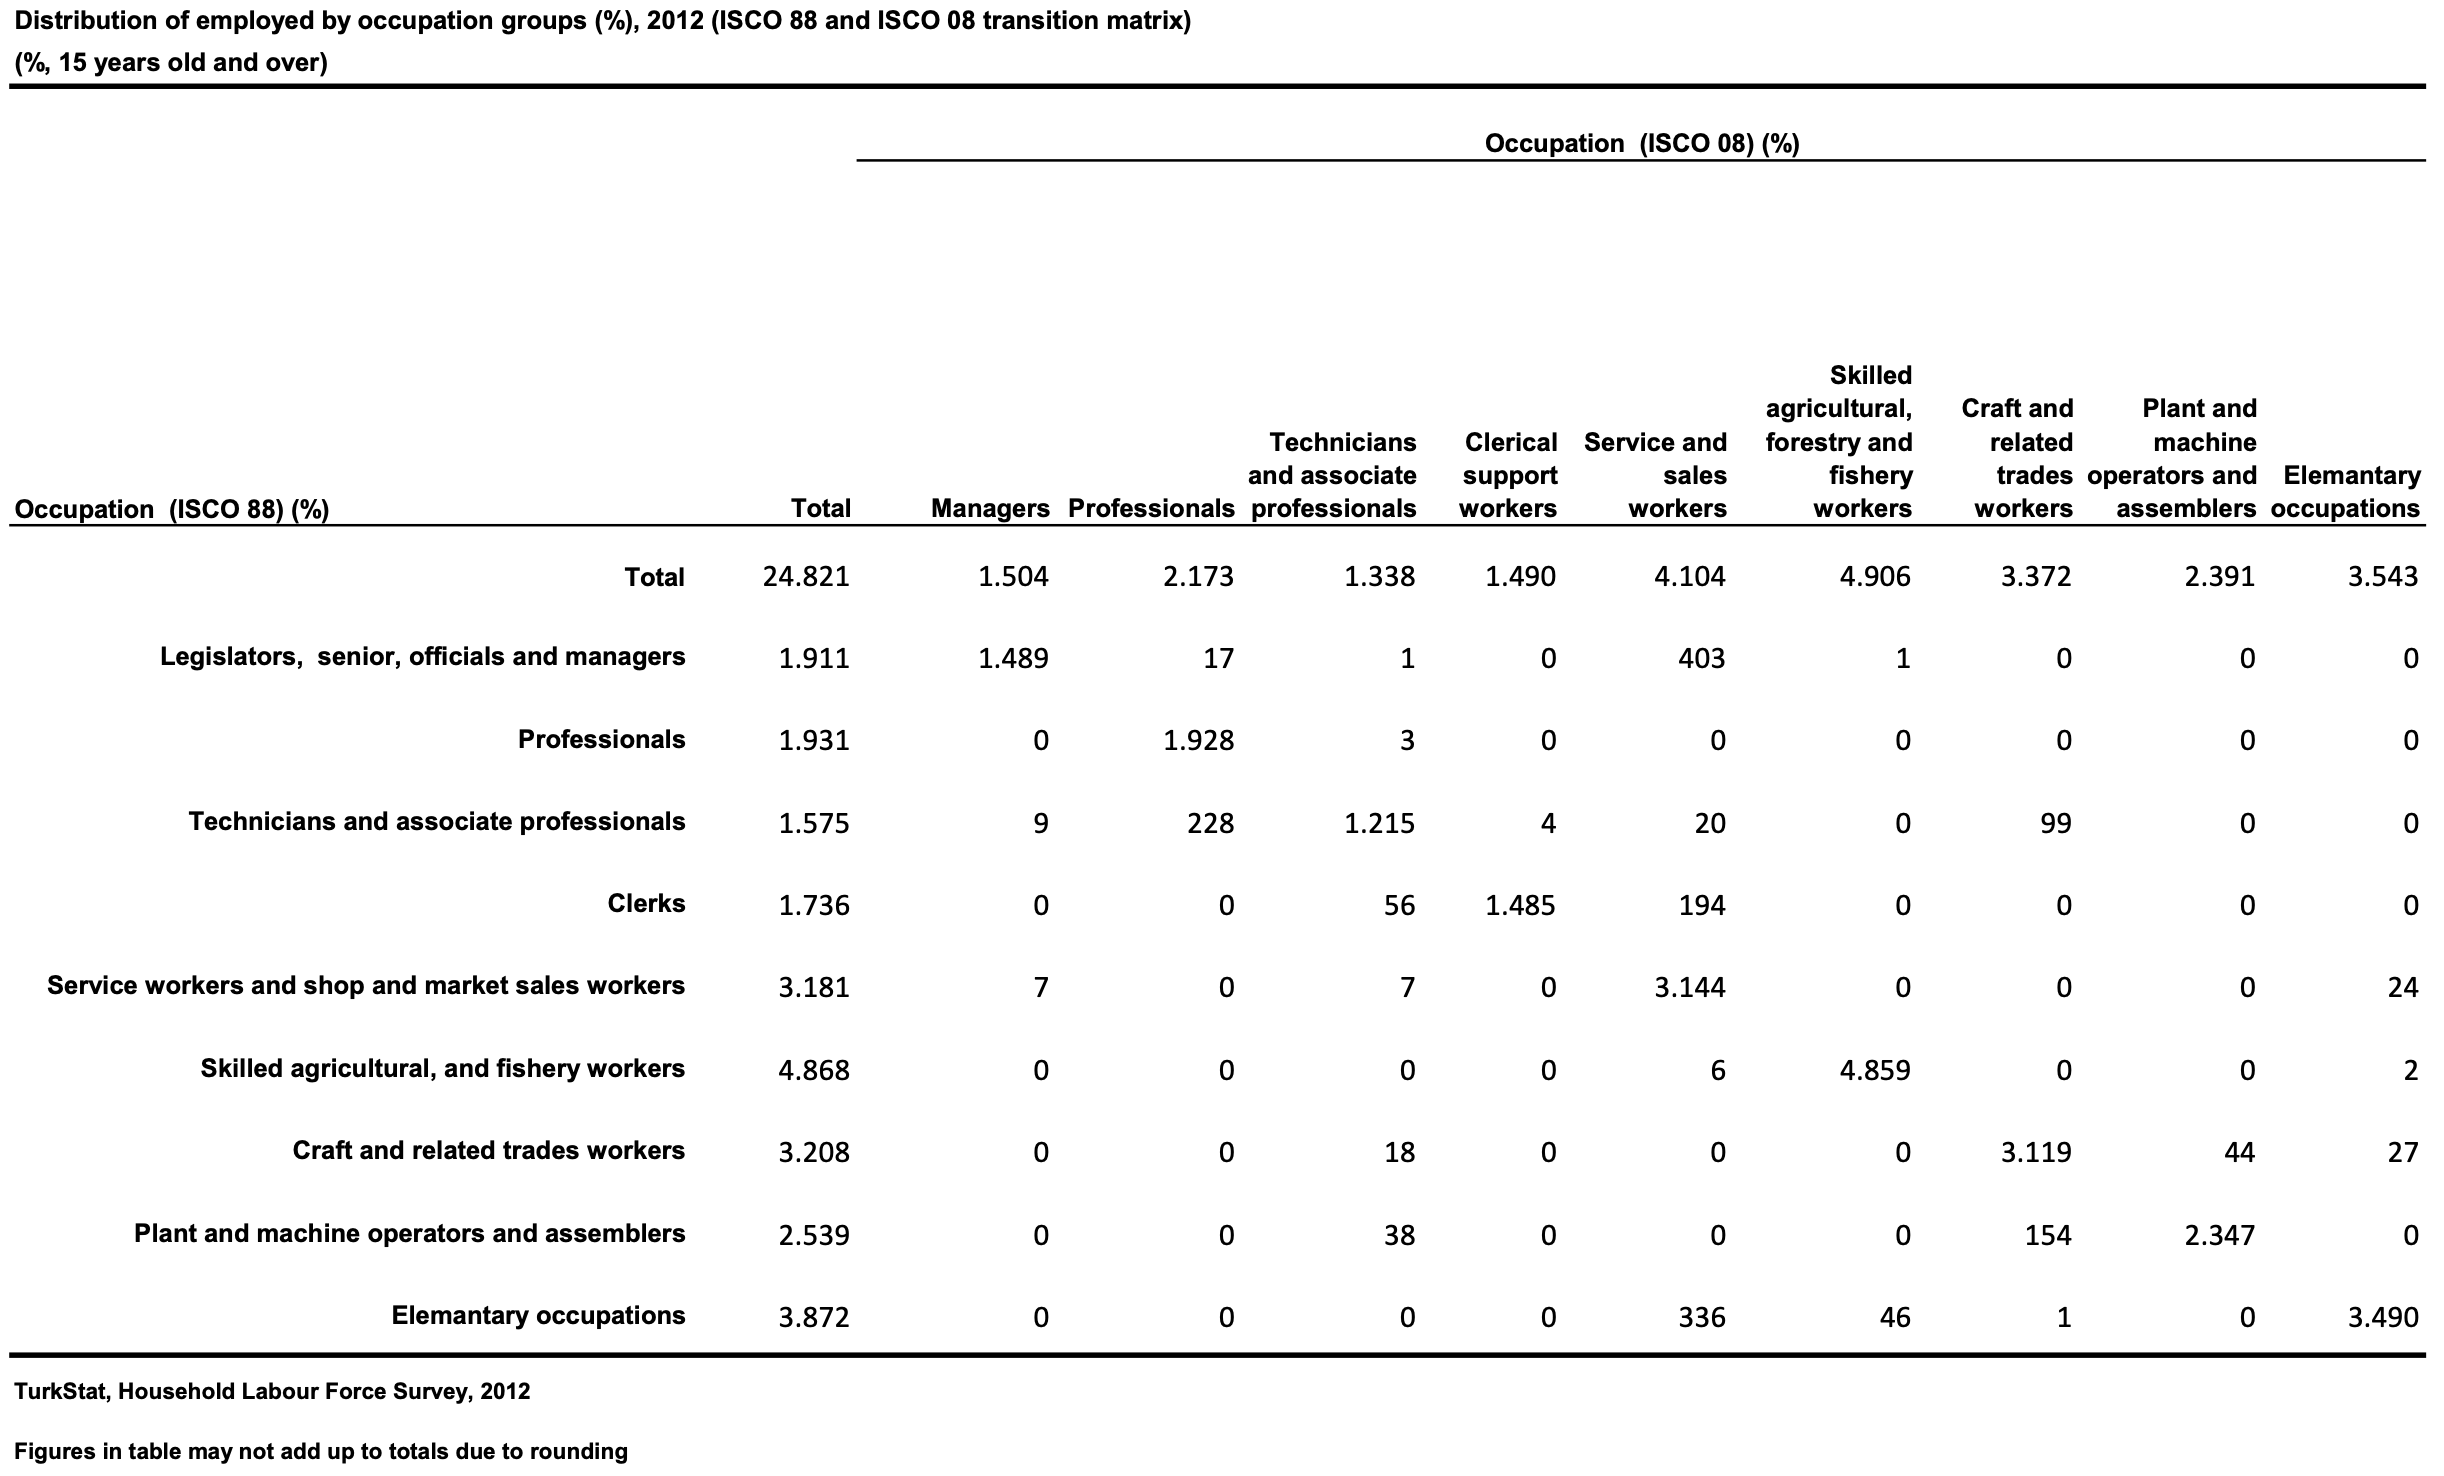
\includegraphics[width=0.8\textwidth]{figs/appendix/isco88-isco08-transition-matrix.png}
\par\end{centering}
\medskip

\begin{singlespace}
\textbf{Source: }2012 HLFS data package from TurkStat.
\end{singlespace}
\end{sidewaystable}

\par\end{center}

\begin{center}
% (hidden draft table moved to extras/unused-content/appendix-hidden-draft.tex)
\par\end{center}
